\documentclass[ruledheader,noindentfirst,anapcustomindent,abntfigtabnum,tocpage=plain]{abnt}
\usepackage{amsmath, amssymb, amsthm, verbatim, amsfonts, amstext}
%\usepackage[latin1]{inputenc}
\usepackage[brazilian]{babel}
\usepackage[utf8]{inputenc}
\usepackage[T1]{fontenc}
\usepackage{dropping}
\usepackage{graphicx}
\usepackage[hang,small,bf]{caption}
\usepackage[abnt-etal-list=0,abnt-etal-text=it,abnt-and-type=&,abnt-emphasize=bf,abnt-full-initials=yes,alf,bibjustif]{abntcite}
\usepackage{fancyhdr}
\usepackage{makeidx}
\usepackage[none]{hyphenat}
\usepackage{color}
\usepackage{subfig}
\usepackage{algorithms}
\usepackage{algorithmic}
\usepackage{mdwlist}
\usepackage{bm}
\usepackage[titletoc,title]{appendix}
\usepackage{ltxtable}
\usepackage{longtable}
\usepackage{supertabular}
\usepackage{indentfirst}
\usepackage{color}
\usepackage{icomma}

\sloppy


%
%Tradução do pacote Algorithm para portugues
%
\renewcommand{\algorithmicrequire}{\textbf{Entrada:}}
\renewcommand{\algorithmicensure}{\textbf{Saída:}}
\renewcommand{\algorithmicend}{\textbf{fim}}
\renewcommand{\algorithmicif}{\textbf{se}}
\renewcommand{\algorithmicthen}{\textbf{então}}
\renewcommand{\algorithmicelse}{\textbf{senão}}
\renewcommand{\algorithmicelsif}{\algorithmicelse \, \algorithmicif}
\renewcommand{\algorithmicendif}{\algorithmicend \, \algorithmicif}
\renewcommand{\algorithmicfor}{\textbf{para}}
\renewcommand{\algorithmicforall}{\textbf{para todo}}
\renewcommand{\algorithmicdo}{\textbf{fazer}}
\renewcommand{\algorithmicendfor}{\algorithmicend \, \algorithmicfor}
\renewcommand{\algorithmicwhile}{\textbf{enquanto}}
\renewcommand{\algorithmicendwhile}{\algorithmicend \, \algorithmicwhile}
\renewcommand{\algorithmicloop}{\textbf{laço}}
\renewcommand{\algorithmicendloop}{\algorithmicend \, \algorithmicloop}
\renewcommand{\algorithmicrepeat}{\textbf{repetir}}
\renewcommand{\algorithmicuntil}{\textbf{até}}
\renewcommand{\algorithmiccomment}[1]{\{#1\}}
\renewcommand{\listalgorithmname}{Lista de Algoritmos}
\floatname{algorithm}{Algoritmo}
%%%%%%%%%%%%%%%%%%%%%%%%%%%%%%%%%%%%%%%%%%%%%%%%%%%%%%%%%%%%%%%%%%%%%%%%%%%%%%%%%%%

\makeindex

%%%% O arquivo modelosCAP.tex possui as definições para ciação do estilo de capítulo (fonte de título, barras horizontais, etc.)
% ele não gera texto de saída, é um arquivo de configuração somente
%
%Estilo de formatação de capítulos

\makeatletter
\newcommand{\thechapterwords}
{ \ifcase \thechapter\or 1\or 2\or 3\or 4\or 5\or6\or 7\or 8\or 9\or 10\or 11\fi}

\def\@makechapterhead#1{%
\vspace*{10\p@}%
{\parindent \z@  \reset@font

\scshape \@chapapp{} \thechapterwords
\quad %
\par\nobreak
\vspace*{10\p@}%
\interlinepenalty\@M
\hrule
\vspace*{10\p@}%
\Huge \bfseries #1\par\nobreak
\par
\vspace*{10\p@}%
\hrule
\vskip 40\p@
}}
\def\@makeschapterhead#1{%
\vspace*{10\p@}%
{\parindent \z@ \centering \reset@font
\par\nobreak
\vspace*{10\p@}%
\interlinepenalty\@M
\hrule
\vspace*{10\p@}%
\Huge \bfseries #1\par\nobreak
\par
\vspace*{10\p@}%
\hrule
\vskip 40\p@
%\vskip 100\p@
}}
%%%%%%%%%%%%%%%%%%%%%%%%%%%%%%%%%%%%%%%%%%%%%%%FIM DO PREAMBULO%%%%%%%%%%%%%%%%%%%%%%%%%%%%%%%%%%%%%%%%%%%%%%%%%%%%%%%%%%%%%%%%%%


\begin{document}

%%%%% IMPORTANTE: ALTERA O TEXTO ENTRE ARIAL E TIMES NEW ROMAN (ALTERNAR OS COMENTÁRIOS)
%
%%%%%%%%%%%%%%%%%%%%%PARA UTILIZAR ARIAL%%%%%%%%%%%%%%%%%%%%%%%
%
\fontfamily{phv}                    %fonte Arial
\renewcommand{\rmdefault}{phv}      %
%
%%%%%%%%%%%%%%%%%%%%%PARA UTILIZAR TIMES%%%%%%%%%%%%%%%%%%%%%%%
%
%\fontfamily{ptm}               %fonte Times
%\renewcommand{\rmdefault}{ptm} %
%
%%%%%%%%%%%%%%%%%%%%%%%%%%%%%%%%%%%%%%%%%%%%%%%%%%%%%%%%%%%%%%%

%%%%%%%%%%%%%Arquivos .tex com os elementos pré-textuais
%
\thispagestyle{empty}

\vfill
 \begin{center}
    \begin{figure}[t]
     \centering
            
\includegraphics[width=5cm]{figures/UFC_logo_sem_t_tulo.png}\\[-0.1in]
     \end{figure}

    {\large\bfseries UNIVERSIDADE FEDERAL DO CEARÁ} \\
    {\large\bfseries CENTRO DE TECNOLOGIA} \\
    {\large\bfseries DEPARTAMENTO DE TELEINFORMÁTICA}  \\ 
    {\large\bfseries CURSO DE ENGENHARIA DE COMPUTAÇÃO}  \\ 

    \vspace*{1in}
    \begin{large} \bfseries PEDRO LUCAS FALCÃO LIMA \end{large}\\[0.4in]

    \vspace*{4cm}
    \noindent \\
    \large\bfseries{Projeto de um IP Soft Core para Detecção de Ataque DDoS} \\
    \vfill
    \large\bfseries{ Fortaleza, Ceará \\ 2017}
\end{center}

\normalsize
\begin{titlepage}
\vfill
\begin{center}

    {\large PEDRO LUCAS FALCÃO LIMA\\}
    \vspace{2cm}
    {\Large \textsc{Projeto de um IP Soft Core para Detecção de Ataque DDoS}\\}
    \vspace{1cm}
    \hspace{.45\linewidth}
    \begin{minipage}{.50\linewidth}

            Monografia submetida à Coordenação de Teleinformática e à Coordenadoria do Curso de Bacharelado 
            em Engenharia de Computação da Universidade Federal do Ceará - Campus do PICI, como requisito 
            parcial para obtenção do grau de Bacharel em Engenharia de Computação.

            \vspace{0.5 cm}

            Área de pesquisa: Utilização de FPGA's 

            \vspace{0.5 cm}

            Orientador: PROF. MSC. JARDEL NUNES DA SILVEIRA
    
    \end{minipage}

    \vspace{2cm}
    \vfill
    {\large Fortaleza\\ 2017}
\end{center}

\end{titlepage}
% ---
% Inserir folha de aprovação
% ---

% Isto é um exemplo de Folha de aprovação, elemento obrigatório da NBR
% 14724/2011 (seção 4.2.1.3). Você pode utilizar este modelo até a aprovação
% do trabalho. Após isso, substitua todo o conteúdo deste arquivo por uma
% imagem da página assinada pela banca com o comando abaixo:
%
% \includepdf{folhadeaprovacao_final.pdf}
%
\begin{folhadeaprovacao}

  \begin{center}
    {\bfseries\Large\imprimirautor}
    \vspace{1cm}

    \begin{center}
      \bfseries\Large\imprimirtitulo
    \end{center}

    \vspace{2cm}
    \begin{minipage}{\textwidth}
        \imprimirpreambulo
        \\ \\ \\
        Aprovada em: \_\_/\_\_/\_\_\_\_
    \end{minipage}%
     
    \vspace{2cm}
	\textbf{BANCA EXAMINADORA}
   \end{center}
	

   \assinatura{\imprimirorientador \space (Orientador) \\ Universidade Federal do Ceará (UFC)}
  
   \assinatura{Prof. Dr. Jarbas Aryel da Silveira \\ Universidade Federal do Ceará (UFC)}
   %DEFINA AQUI OS DEMAIS MEMBROS DA BANCA
   \assinatura{Prof. Dr. Otávio Alcântara de Lima Júnior \\ Instituto Federal do Ceará - IFCE}
   %\assinatura{Prof. Dr. Alguma Coisa \\ Instituição}
   %\assinatura{Prof. Msc. Alguma Coisa \\ Instituição}
     
%   \begin{center}
%    \vspace*{0.5cm}
%    {\large\imprimirlocal}
%    \par
%    {\large\imprimirdata}
%    \vspace*{1cm}
%  \end{center}
  
\end{folhadeaprovacao}
% ---
% ---
% Dedicatória
% ---
\begin{dedicatoria}
   \vspace*{\fill}
   	\begin{flushright}
   \noindent
    Dedico este trabalho à minha família e namorada, pessoas que \\fizeram de tudo para que eu chegasse onde cheguei.
   	\end{flushright}
\end{dedicatoria}
% ---
% ---
% Agradecimentos
% ---
\begin{agradecimentos}
	Agradeço primeiramente a Deus, por sempre ter guiado meus passos e ter me dado saúde e força para superar as dificuldades.
	
	Aos membros da minha família, pelo amor e apoio em todos os momentos, principalmente minha Mãe, Lenilce, e minha vó, Julia, pela educação e pelos conselhos que me ajudaram a ser quem sou hoje.
	
	À minha namorada, Fernanda Meyre, pelo amor, apoio e compreensão nos momentos de dificuldade.
	
	Ao meu orientador, Prof. Dr. Emanuel Bezerra Rodrigues, pela oportunidade de conhecer o ramo de pesquisa em telecomunicações, pelo apoio, incentivo, sugestões e comentários durante a supervisão dos meus estudos.
	
	Ao meu coorientador, Prof. Dr. Tarcísio Ferreira Maciel, pelo apoio, incentivo, sugestões e tempo dedicado para me ajudar durante meus estudos.
	
	Aos professores, Prof. Dr. Helano Sousa Castro, Prof. Dr. George André Pereira Thé e Profa. Dra. Fátima Nelsizeuma Sombra de Medeiros, pelos ensinamentos técnicos e conselhos. 
	
	Aos meus amigos da Universidade Federal do Ceará, University of British Columbia e do Grupo de Pesquisa em Telecomunicações sem Fio (GTEL) pela amizade e pelos momentos de descontração e estudo.
	
	E a todos que direta ou indiretamente fizeram parte da minha formação, o meu muito obrigado.
\end{agradecimentos}
% ---
% ---
% Epígrafe
% ---
\begin{epigrafe}
    \vspace*{\fill}
	\begin{flushright}
		\textit{"A persistência é o caminho do êxito."\\
		(Charles Chaplin)}
	\end{flushright}
\end{epigrafe}
% ---
\pagestyle{plain}%%%%% Utilizar ESTILO PLAIN AQUI%%%%%%%
\chapter*{Resumo}

\noindent Este trabalho apresenta...
\chapter*{Abstract}


\noindent This work presents...

%%%Comandos para criação automática das listas
%
\tableofcontents
\listoffigures
\listoftables

%%%Comandos para criar outras listas não suportadas pelo pacote ABNTex%%%
%
\pretextualchapter{Lista de Símbolos}
\begin{basedescript}{\desclabelstyle{\pushlabel}\desclabelwidth{6em}}
\item[$Z$] variavel aleatoria%
\item[$\mathbb{R}$] conjunto dos números reais%
\item[$t$] tempo contínuo%
\item[$n$] tempo discreto%
\item[$f(z)$] função densidade de probabilidade%
\item[$F(z)$] função de distribuição acumulada%
\item[$\sigma$] desvio padrão%
\item[$\mu$] média ou esperança matemática%
\item[$|\cdot|$] operador magnitude%
\item[$\nabla$] operador gradiente%
\end{basedescript}
\newpage

\pretextualchapter{Lista de Abreviacoes}
\begin{basedescript}{\desclabelstyle{\pushlabel}\desclabelwidth{6em}}
\item[{fdp}] Função densidade de probabilidade%
\item[{fda}] Função de distribuição acumulada%
\item[{EMQ}] Erro médio quadrático%
\end{basedescript}
\newpage
%%%%%%%%%%%%%%%%%%%%%%%%%%%%%%%%%%%%%%%%%%%%%%%%%%%%%%%%%%%%%%%%%%%%

%Capítulos passam a ter páginas numeradas
%
\pagestyle{fancy}

%resseta os contadores de capítulo e seção
%
\renewcommand{\chaptermark}[1]{\markboth{#1}{}}
\renewcommand{\sectionmark}[1]{\markright{\thesection\ #1}}

%%%%%%%%%%%%%%NÃO LEMBRO O QUE FAZ, APARENTEMENTE NADA, TESTAR DEPOIS
%\fancyhf{}%
%\fancyhead[RO,LE]{\large\slshape\thepage}%
%\fancyhead[CE]{\large\slshape\leftmark}%
%\fancyhead[CO]{\large\slshape\rightmark}%


%%% Outros arquivos .tex. É acoselhável utilizar vários arquivos, pelo menos um por capítulo
\chapter[Introdução]{Introdução}
\label{introducao}
% ---------------------------------------------------------
Com a crescente difusão da \textit{internet} e sistemas \textit{web} na
atualidade, cada  vez mais serviços são disponibilizados por meio da rede mundial de computadores. Serviços tais como armazenamento, transações financeiras e plataformas de dados cadastrais são cada vez mais comuns. Por isso, é necessário que tais serviços cumpram os requisitos de disponibilidade e segurança. Assim, sistemas de detecção de intrusão (IDS), são comumente usados para garantir a segurança por meio de análise e detecção de tráfegos maliciosos,bem como tomar medidas corretivas em caso de tráfegos maliciosos.

Mediante a esse crescimento de usuários e serviços na \textit{internet}, ameaças na rede vem desenvolvendo-se cada vez mais. Por isso, nota-se uma maior complexidade nessas ameaças. De acordo com \citeonline{mandia2001hackers} são considerados ataques a segurança quaisquer eventos que interrompam os procedimentos normais causando algum nível de crise, tais como invasões de computador, ataques de negação de serviço, furto de informações por pessoal interno. Ataques podem ser do tipo de negação de serviços.

Os ataques \textit{DoS} (sigla para Denial of Service), que podem ser interpretados como "Ataques de Negação de Serviços", consistem em tentativas de fazer com que computadores - servidores \textit{Web}, por exemplo tenham dificuldade ou mesmo sejam impedidos de executar suas tarefas. Para isso, em vez de "invadir" o computador ou mesmo infectá-lo com \textit{malwares}, o autor do ataque faz com que a máquina receba tantas requisições que esta chega ao ponto de não conseguir dar conta delas. Em outras palavras, o computador fica tão sobrecarregado que nega o serviço \cite{HOQUE201748}. Ataques do tipo \textit{DoS} distribuidos são chamados de ataques \textit{DDoS}.

 \textit{DDoS}, sigla para \textit{Distributed Denial of Service}, é um tipo de ataque  \textit{DoS} de grandes dimensões, ou seja, que utiliza até milhares de computadores para atacar uma determinada máquina, distribuindo a ação entre elas. Trata-se de uma forma que aparece constantemente no noticiário, já que é o tipo de ataque mais comum na \textit{internet} \cite{alecrim2008ataques}.
	
Para detectar ataques  \textit{DDoS} em tempo real, o mecanismo de detecção deve ser capaz de detectar ataques de forma eficiente de um pequeno conjunto de características relevantes.
Portanto, é necessária uma medida efetiva  para classificar um  tráfego em tempo real. 

Essa detecção passa, por uma série de análises de dados, por isso é necessário a utilização de medidas estatísticas, consequentemente cálculos computacionalmente complexos. O alto rendimento é essencial para a escalabilidade da detecção , o que é necessário no caso de ataques \textit{DDoS}.

Diante disso, soluções baseadas em software são ineficientes para aplicações de tempo real, uma vez que eles exigem grande quantidade de ciclos de \textit{CPU} de propósitos gerais. Logo, é necessário que soluções em \textit{hardware} estejam presentes nas detecções de ataques \textit{DDoS} . Podendo assim, ser gerados sistemas híbridos (\textit{hardware} e \textit{software}) que possuem alto desempenho e precisão.

Os tipos de Hardware que possuem características para acomodar grandes lógicas e possuem alto desempenho são as \textit{FPGAs} e \textit{ASICs}, porém as \textit{FPGAs} oferecem adaptabilidade dinâmica, que é importante para aplicações que requerem mudanças frequentes em suas configurações, como a detecção de ataques \textit{DDoS} que evoluem com frequência. 

Por isso foi proposto um módulo de detecção , afim de garantir desempenho e precisão de ataques, utilizando \textit{FPGA}, que junto a sistemas de  \textit{softwares} consigam detectar ataques  \textit{DDoS}.

\section{Objetivos}

   Este trabalho tem os seguintes objetivos gerais e específicos.
\subsection{Objetivos Gerais}
\begin{itemize}

\item  A implementação de um módulo em hardware capaz de detectar de ataques em tempo real.

\item  A implementação de um módulo em hardware que possua um ganho de desempenho e possua precisão satisfatória em relação a módulos em softwares.

\item Ganhos de desempenho em relação a trabalhos similares.	

\end{itemize}

\subsection{Objetivos Específicos}
\begin{itemize}
	
	\item  Estudo de métodos que utilizam aproximação aos resultados de cálculos em softwares de maneira otimizada.
	
	\item A Utilização de IP cores no desenvolvimento, para uma maior agilidade e confiabilidade na construção do código. 
	
\end{itemize}
\section{Organização da monografia}
Este documento está organizado da seguinte forma: No \capref{fundamentacao} é apresentado um estudo bibliográfico sobre ameaças de rede e ataques \textit{DDoS},detecção e solução em \textit{hardware}. No \capref{metodologia}, a modelagem do módulo Nahid é descrita e no \capref{resultados}, apresentamos os resultados  do módulo implementado por meio da taxa de correlação calculada na detecção e tempo de computação de detecção. Por fim, o último capítulo deste trabalho apresenta as conclusões realizadas a partir dos resultados obtidos, além de algumas perspectivas para a continuação deste trabalho.
\chapter{Métodos de Kernel}
\label{CAP2}


Este capítulo tem como objetivo 


\section{Kernel em análise de padrões}\label{Sub:equa}

Em análise de padrões, temos como objetivo detectar automaticamente padrões em um conjunto de dados de um determinado problema. Por padrões, podemos entender qualquer relação ou regularidades inerentes à alguma estrutura em uma fonte de dados. Essa análise geralmente é feita a partir dos valores de entrada e suas respectivas saídas(no caso da aprendizagem supervisionada) fornecidas no problema. Essas informações podem formar padrões em que se torna possível verificar o valor de uma saída dada uma nova entrada fornecida pelo usuário. 

Diversos problemas podem ser resolvidos utilizando esta abordagem, categorização de textos, análise de sequências de DNA, reconhecimento de escrita, por exemplo.

A abordagem de análise de padrões utilizando métodos de kernel se baseia em adaptar os dados de entrada em um espaço característico adequado e nos algoritmos usados para descobrir os padrões do problema. Levando em conta isso, podemos pensar que qualquer solução com métodos de kernel é composta por estas duas partes: uma em que é feito o mapeamento nesse espaço característico e a outra em que é executado o algoritmo de aprendizagem para detectar os padrões neste espaço. A ideia por trás desta abordagem é poder mapear os dados em um espaço em que possamos 

Uma das principais caracerísticas desses métodos é o atalho computacional que pode ser utilizado, tal atalho é conhecido como função de kernel.


O Kernel  é uma função de mapeamento de dados em dimensões superiores com a motivação de torná-los mais fáceis de separar ou estruturá-los de maneira mais adequada. Essas funções podem ser utilizadas nas tarefas de reconhecimento de padrões. 

\begin{equation}\label{Eq:multiplicacao}
%
Z = X \cdot Y,
%
\end{equation}
%
em que $Z$, $X$ e $Y$ são variáveis complexas. A referenciação à Equação (\ref{Eq:multiplicacao}) é feita por meio do comando ``ref''. O mesmo vale para outros tipos de elementos.

\subsection{Exemplo de uma equação mais complexa}

  Equações mais complexas podem ser mais facilmente escritas com uso do programa TexAide. Como, por exemplo,

    \begin{equation}\label{Eq:sqrt_gamma_X}
    f_{\Gamma ^{{1 \mathord{\left/
    {\vphantom {1 2}} \right.
    \kern-\nulldelimiterspace} 2}} } (x;\alpha ,\lambda ) = \frac{{2\lambda ^\alpha  }}{{\Gamma (\alpha )}}x^{2\alpha  - 1} \exp \left( { - \lambda x^2 } \right).
    \end{equation}
    \[
    \alpha ,\lambda > 0.
    \]
    %
    em que $\Gamma(\cdot)$ é a função Gama. O programa TexAide é semelhante ao \textit{MathType} do Office, porém ao copiar e colar a equação em um arquivo tex, é gerado o código em LaTex referente a esta equação.

\section{Tabelas}

Tabelas são essenciais na apresentação de dados. A Tabela \ref{Tb:X_models} mostra um exemplo do uso deste tipo de elemento. Vale ressaltar que não é aconselhável o uso de linhas verticais em trabalhos acadêmicos e de pesquisa.

\begin{table}[h]
 \caption{Modelos estatísticos e suas relações.}%
 \label{Tb:X_models}
  \centering
\begin{tabular}{c c c c c}
 \hline
 &&&&\\
                                             &$\alpha ,\lambda  > 0$    &                               &$\alpha ,\lambda \rightarrow\infty$  &Homogêneo \\
                                             &$\gamma  \to 0$           & Heterogêneo                   &$\alpha / \lambda \rightarrow \beta$ & \\
                                             &$\mathop  \to \limits^D $ & $\sqrt\Gamma(\alpha,\lambda)$ &$\mathop  \to \limits^P $            &$\sqrt\beta$        \\
$\mathcal{N}^{-1/2}(x;\alpha,\gamma,\lambda)$& & & &\\
                                             &$\mathop  \to \limits^D $ & $\Gamma^{-1/2}(\alpha,\gamma)$&$\mathop  \to \limits^P $   &$\sqrt{\zeta^{-1}}$ \\
                                             &$\lambda \to 0$           &  Extremamente                 &$-\alpha / \gamma \rightarrow \zeta^{-1}$ & \\
                                             &$-\alpha ,\gamma   > 0$   &  Heterogêneo                  &$-\alpha ,\gamma \rightarrow\infty$ &Homogêneo \\
 &&&& \\
 \hline
 &&&&\\
                                             &$\alpha ,\lambda  > 0$    &                               &$\alpha ,\lambda \rightarrow\infty$  &Homogêneo \\
                                             &$\gamma  \to 0$           & Heterogêneo                   &$\alpha / \lambda \rightarrow \beta$ & \\
                                             &$\mathop  \to \limits^D $ &$\mathcal{K}_A(\alpha,\lambda,n)$&$\mathop  \to \limits^P $&$\sqrt\Gamma(n,n/\beta)$        \\
$\mathcal{G}_A(z;\alpha,\gamma,\lambda,n)$   & & & &\\
                                             &$\mathop  \to \limits^D $ & $\mathcal{G}_A^0(\alpha,\gamma,n)$&$\mathop  \to \limits^P $&$\sqrt\Gamma(n,n\zeta)$  \\
                                             &$\lambda \to 0$           &  Extremamente                 &$-\alpha / \gamma \rightarrow \zeta$ & \\
                                             &$-\alpha ,\gamma   > 0$   &  Heterogêneo                  &$-\alpha ,\gamma \rightarrow\infty$ &Homogêneo \\
&&&&   \\
 \hline

\end{tabular}
\end{table}


A Figura \ref{Fig:1} mostra o exemplo do uso do comando ``subfigure''. Apesar de aceitar diferentes tipos de imagens. É preferível que as imagens estejam no formato .eps. Isso garante que a imagem impressa seja exatamente aquela visualizada, como acontece com arquivos pdf.

\begin{figure}[!ht]
\centering
\subfloat[]{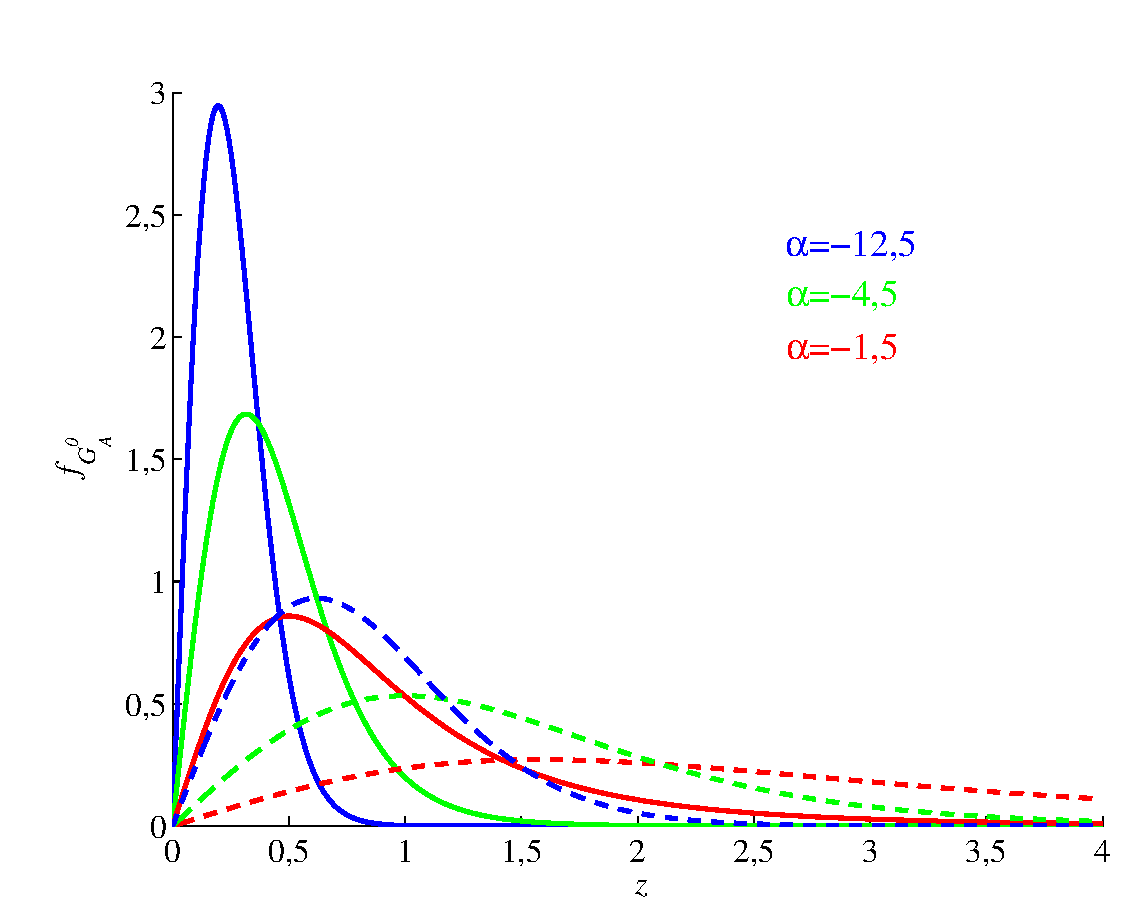
\includegraphics[scale=.65]{figures/fig1.eps}}\\
\subfloat[]{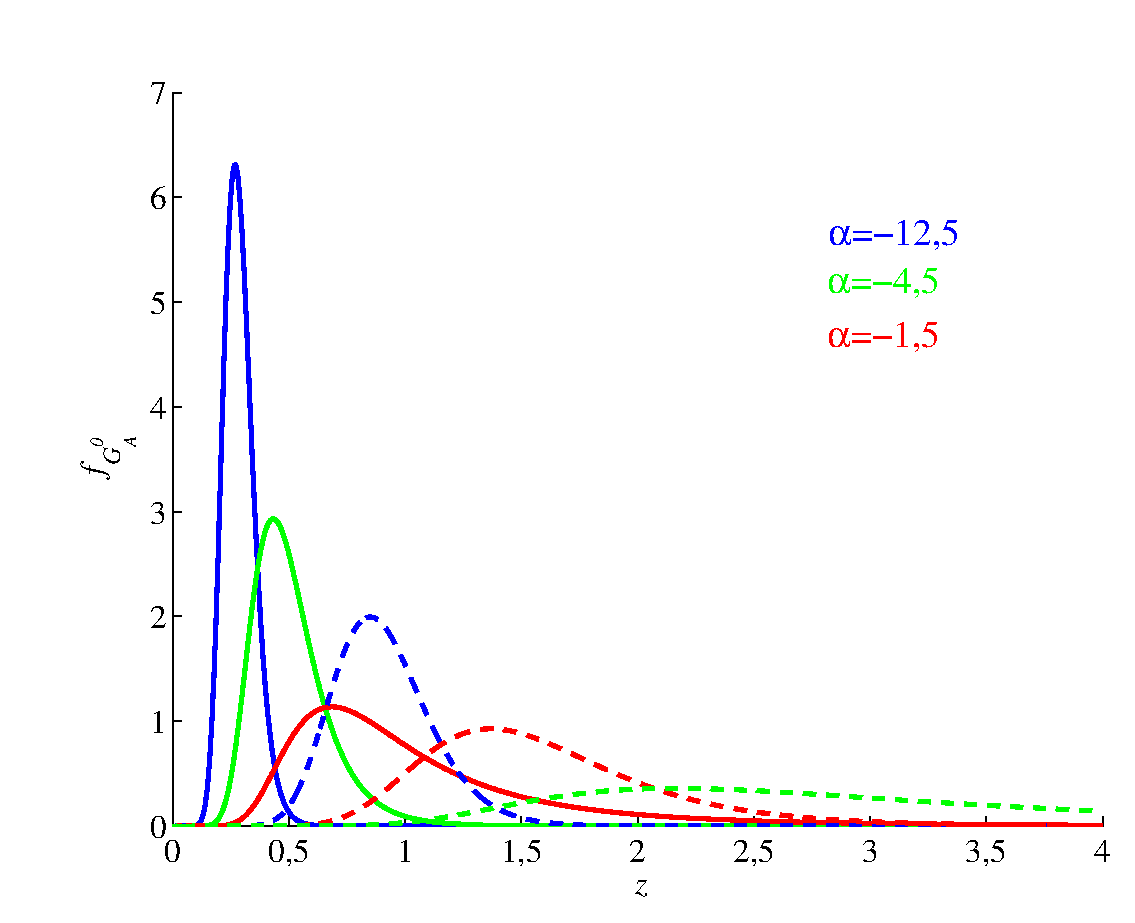
\includegraphics[scale=.65]{figures/fig2.eps}}
\caption{ Curvas de funções de probabilidade: (a) exemplo 1, (b) exemplo 2.} \label{Fig:1}
\end{figure}
\chapter{Módulo Nahid}
\label{CAP3}

O  módulo de detecção em hardware é basicamente a implementação da formulação dos passos da correlação proposta, utilizando uma FPGA. Para isso, é necessário adequar  as operações para os componentes que são disponíveis e escolhidos para realizar a computação de uma dada operação.  Além disso, para otimizar o tempo de resposta é necessário uma organização dessas operações em ciclos de clock, para ter uma referência de tempo  para cada computação realizada e assim organizar a sequência das operações. Com isso , a arquitetura de detecção de ataques é proposta com o nome de Nahid. Essa arquitetura possui componentes de diversos níveis, nos quais estão dispostos dependendo da operação que esteja sendo feita no momento, vale ressaltar que essas operações são aritméticas, mudança no tamanho da palavra, registro e seleção.  

\section{Módulo Nahid}\label{Sub:equa}

Nahid é o componente de mais alto nível, sendo ele quem recebe as entradas(perfil normal e instâncias de tráfego em análise) do módulo pré-processador e envia a saída (resultado da análise) para gerenciador de segurança. O Nahid é composto basicamente por dois componentes  internos, esses são: Datapath e Controller.  Além dos vetores de entrada citados anteriormente, o componente  Nahid recebe os sinais de controle clock e start (que serão os sinais que indicaram início da detecção e as mudanças de ciclos). Esse componente  abstrai toda a combinação lógica que foi implementado nos componentes  internos, porém é de suma importância para realizar a junção de entradas e saídas entre componentes internos, módulos e  gerenciadores. 
  \begin{figure}[t]
	\centering
	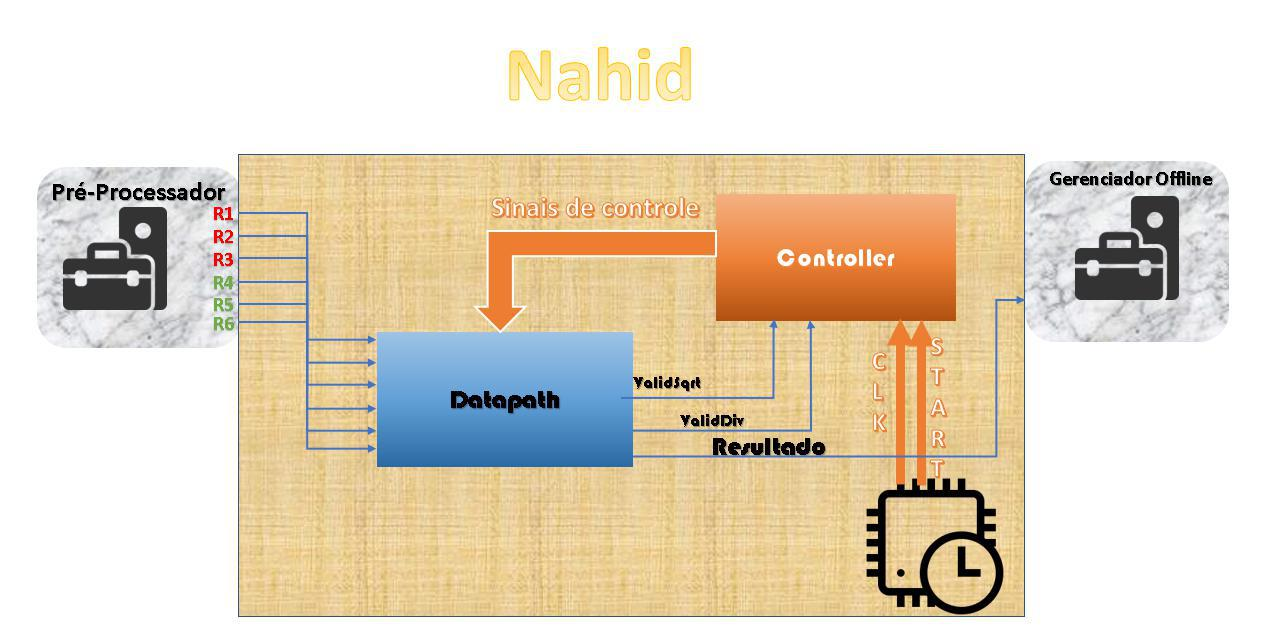
\includegraphics[width=12cm]{figures/nahid.jpg}\\
\end{figure}

\subsection{Datapath}

O componente responsável por alocar todos os componentes que realizam as operações da detecção  é o Datapath. Por isso, o mesmo comporta no mínimo um dos componentes de mais baixo nível, que serão descritos posteriormente. O Datapath recebe os vetores de entradas(perfil normal e instâncias de tráfego em análise) do Nahid, pois esses dados são selecionados, tratados e registrados pelos componentes internos do Datapath. Porém para isso é necessário que seja indicado ao componente quais são as entradas a serem processadas num dado ciclo, por isso o Datapath recebe como entrada seletores provindos do Controller . Entretanto , o Datapath possui saídas para o controller, pois em alguns ciclos é necessário de alguma confirmação de algum componente  interno ao Datapath, além disso a saída do sistema será um resultado registrado num componente interno e será em enviado ao componente de mais alto nível (Nahid).
\subsubsection{Extend}
Esse componente possui a função de estender o tamanho de uma palavra de bits de qualquer tamanho (menor que 23), para uma palavra de mesmo conteúdo com tamanho de 23 bits. Esse componente é de suma importância nas operações de soma, uma vez que o componentes de soma (Adder) possuem entradas de tamanho de 23 bits. O Datapath possui 12 componentes do tipo extend. Esse componente é do tipo de mudança no tamanho da palavra e em um ciclo ele completa sua computação.	
\subsubsection{Reduce}
Esse componente possui a função de reduzir o tamanho de uma palavra de bits de qualquer tamanho (maior que 11), para uma palavra de mesmo conteúdo com tamanho de 11 bits. Esse componente é de suma importância nas operações de multiplicação, uma vez que o componentes de multiplicação( Mul) possuem entradas de tamanho de 11 bits. O Datapath possui 4 componentes do tipo reduce. Esse componente é do tipo de mudança no tamanho da palavra e um em ciclo ele completa sua computação.	
\subsubsection{Mux}
Esse componente possui a função de ter na entrada vários opções, porém a cada iteração, existe um seletor que indica que entrada será utilizada num dado momento, levando para saída do componente essa escolha. Esse componente é de suma importância para reutilização de componentes, deixando a arquitetura mais enxuta e coesa, sendo muito utilizado no Controller, pois para cada ciclo existem determinadas escolhas nesses multiplexadores. É importante ressaltar, que no Datapath existem mux de diversos tamanhos (2 entradas,4 entradas e 6 entradas), isso está diretamente relacionado com o componente que recebe a saída do mux, pois quanto mais ele pode ser utilizado por entradas diferentes, maior será o número de entradas no multiplexador combinado a esse componente. Devido aos multiplexadores terem grande importância na reutilização de componentes, existem duas frentes de alocação de mux no Datapath. Nas operações aritméticas(Multiplicadores e Somadores) e de registro(Registradores). Esse componente é do tipo de seleção de dados e em um ciclo ele completa sua computação.	
\subsubsection{Mul}
Esse componente possui a função de receber duas entradas, e realizar a multiplicação aritmética das mesmas, gerando uma saída do resultado. Foi utilizado um Mul que recebe entradas de 11 bits podendo gerar até 22 bits no resultado dessa multiplicação. Existem 3 multiplicadores no Datapath, que em nosso módulo realizam operação de quadrado de um número, ou seja as multiplicações tem as mesmas entradas num dado momento. Esse componente é do tipo operações aritméticas e em ciclo ele completa sua computação e em um ciclo ele completa sua computação.
\subsubsection{Adder}
Esse componente possui a função de receber duas entradas, e realizar a soma aritmética das mesmas, gerando uma saída do resultado. Foi utilizado um adder que recebe entradas de 23 bits podendo gerar até 24 bits no resultado dessa soma. Vale ressaltar que o componente possui 4 modos de operação, o que caracteriza diferentes formas de somar as entradas. Esses modos são:
\begin{itemize}
\item O modo 0: A soma padrão de dois números positivos.
\item O modo 1: A soma de dois números positivos, com o resultado dividido por 4.
\item O modo 2: O módulo de dois números positivos
\item O modo 3: O módulo de dois números positivos, com o resultado dividido por 4.
\end{itemize}

Esses modos de operação, são necessários pelos diversos “cálculos” que são necessários na formulação da correlação que o módulo implementa, por isso algum componente é necessário implementar essas adições, sendo escolhido o Somador.
Existem 5 somadores no Datapath, que no módulo realizam operações de adição necessárias. Vale ressaltar que o seletor de operação, também é uma entrada do Adder. Esse componente é do tipo operações aritméticas e em um ciclo ele completa sua computação.
\subsubsection{Divider}
Esse componente possui a função de receber duas entradas, e realizar a divisão aritmética das mesmas, gerando uma saída do resultado. Esse componente possui certas peculiaridades, pois uma divisão em hardware é mais custosa, pela existência de números fracionários nos resultados de divisões decimais, que interferem diretamente nas operações e no resultado do módulo. Por isso existe a necessidade da utilização de alguma representação numérica que possa trazer resultados fracionários, foi utilizado nesse caso representação em ponto fixo como falado anteriormente. O componente Divider utilizado foi o IP core da xilinx “Divider Generator”, que foi configurado da seguinte forma: 
\begin{itemize}
\item 	Dividendo: 12 bits
\item 	Divisor: 12 bits
\item 	Quociente: 12 bits
\item 	Parte Fracionária: 8 bits
\end{itemize}
Em outras palavras, temos 2 entradas de 12 bits e uma saída de 20 bits, porém na representação de ponto fixa, tem-se 12.8(12 números na parte inteira e 8 na decimal). Além dessas instâncias, existem dois sinais de controle no módulo, o” valid in” (responsável por indicar que o componente está pronto para receber as entradas e iniciar a computação) e o “valid out” (responsável por indicar que o componente acabou de realizar a operação por completo e já tem o resultado), esses sinais são de suma importância para a organização do módulo e regulação dos ciclos. Existe apenas um componente do tipo do Divider, que realiza divisões que não possuem divisor diferente de potências de 2 (pois pode-se utilizar mecanismos mais simples, para realizar essas divisões, mantendo o resultado no universo dos inteiros).  Esse componente é do tipo operações aritméticas e em 22 ciclos ele completa sua computação.
\subsubsection{Sqrt}
Esse componente possui a função de receber uma entrada, e realizar a raiz quadrada aritmética da mesma, gerando uma saída do resultado. Esse componente possui resultados inteiros, porém o resultado é um inteiro aproximado para números que não possuem raízes fechadas, pois é possível os números de entradas não serem quadrados perfeitos e o resultado da raíz ser número com casas decimais. Para realizar a busca e aproximação de resposta, é necessário algum algoritmo de busca dessa raiz, gerando um certo custo de ciclos, como no divisor. Para tal o componente Sqrt utilizado foi o IP core da xilinx “Cordic” (função Raíz), que foi configurado da seguinte forma: 
\begin{itemize}
\item Entrada: 22 bits
\item Saída: 12 bits
\end{itemize}
Logo, temos 1 entrada de 22 bits e uma saída de 12 bits. Além dessas instâncias, existem dois sinais de controle no módulo, o” valid in” (responsável por indicar que o componente está pronto para receber a entrada e iniciar a computação) e o “valid out” (responsável por indicar que o componente acabou de realizar a operação por completo e já tem o resultado), esses sinais são de suma importância para a organização do módulo e regulação dos ciclos. Existe apenas um componente do tipo do Sqrt, esse componente é do tipo operações aritméticas e em 6 ciclos ele completa sua computação.

\subsubsection{Register}
Esse componente possui a função de receber uma entrada, e armazenar o valor recebido a partir da próxima subida do clock e atualizar o valor que estiver na entrada na próxima subida do clock. De forma que pelomenos durante um ciclo o registrador terá o valor recebido num dado momento, por isso podemos considerar o conjunto de registradores como a memória do módulo. Os registradores são de suma importância para a realizar as operações, uma vez que não para realizar todos os passos da correlação, “guardam-se” variáveis de uma operação para utilizar nas próximas operações. O Registrador implementado por padrão recebe entradas de 24 bits e a saída tem o mesmo tamanho, porém existem registradores específicos que possuem tamanhos diferentes do padrão, por serem usados para em fins específicos. Além da entrada, o Registrador recebe o sinal “enable” (responsável para habilitar ou não o registro do componente, no próximo ciclo de clock) e “clr” (responsável por zerar o registro do componente, no próximo ciclo de clock). Existem 11 registradores no Datapath, que realizam o regsitro necessários no módulo. Esse componente é do tipo registro e em um ciclo ele completa sua computação.
\subsection{Controller}
O componente responsável por organizar os ciclos das operações do Módulo Nahid é o Controller. Quais componentes do Datapath que serão utilizados num determinado ciclo de computação e em que ciclo teremos os resultados de uma dada operação, são as principais funções desse componente. O Controller recebe o clk (clock do sistema) e o start (sinal que indica o início do módulo) do Nahid, para que o componente garante que o sistema está síncrono. Além dessas entradas, como dito anteriormente, recebe os sinais “valid out” dos componentes Divider e Sqrt. O Controller possue saídas para o Datapath, para indicar a esse componente o que será utilizado num dado ciclo. A estrutura do controller pode ser dividida em dois cases:
\begin{enumerate}
\item Case de operações: Esse case é responsável por indicar todas as operações que serão feitos em todos os ciclos. 
\item Case de transições de ciclos: Esse case é responsável por indicar quando haverá as transições de um ciclo para outro.
\end{enumerate} 
\chapter{Resultados Experimentais}\label{CAP4}

\begin{table}[!htb]
   \centering
\caption{Relatório de Utilização}
\label{Tab:teste}
\begin{tabular}{lcccc}
	\hline
\multicolumn{1}{c}{Tipo}&\multicolumn{1}{c}{Usado}&\multicolumn{1}{c}{Fixo}&\multicolumn{1}{c}{Disponível}&\multicolumn{1}{c}{Utilização\%} \\ \midrule
 CLB LUTs*&  1302  & 0 & 216960 & 0.60  \\   \midrule
 LUT as Logic & 1301 & 0 & 216960 &  0.60  \\  \midrule
 LUT as Memory &  1 & 0 & 99840 &  <0.01  \\  \midrule
 LUT as Distributed RAM &0 & 0 &  &   \\  \midrule
 LUT as Shift Register & 1 & 0 &  &   \\  \midrule
 CLB Registers  & 1180 & 0 & 433920 & 0.27  \\  \midrule
 Register as Flip Flop & 1122 & 0  & 433920  &  0.26    \\  \midrule
 Register as Latch & 58 & 0 & 433920  &  0.01  \\  \midrule
 CARRY8 & 78 & 0 & 27120 & 0.29  \\  \midrule
 F7 Muxes &0 & 0 & 108480 &  0.00   \\  \midrule
 F8 Muxes & 0 &0 & 54240 &  0.00  \\  \midrule
 F9 Muxes & 0 & 0 & 27120 &  0.00 \\  \midrule
\end{tabular}
\end{table}

 





\chapter{Conclusão e Trabalhos Futuros}\label{CAP5}


%%%% Estilo de citação ABNT e arquivo de bibitens (mybibliography.bib)
\bibliographystyle{abnt-alf}
\bibliography{mybibliography}

\apendice
\chapter{Título do Apêndice}
\label{Apx:A}




\chapter{Exemplo do pacote Algorithm}
\label{Apx:B}


\begin{algorithm}[!h]
\caption{Estimador ML otimizado.}\label{Alg:MAXVER}
\begin{algorithmic}[1]
\STATE Inicializar o contador: $j\leftarrow 1$;%
\STATE Fixar o limiar de variação das estimativas: $e_{\mathrm{out}}\leftarrow 10^{-4}$;%
\STATE Fixar o número máximo de iterações: $N\leftarrow 1000$;%
\STATE Computar o ponto inicial: $\hat \gamma(0)$;%
\STATE Determinar o limiar inicial: $e_1 \leftarrow1000$;%
\STATE Estabelecer o valor inicial de $\alpha$: $\hat \alpha(0) \leftarrow -10^{-6}$;%
\WHILE{ $e_j \geq e_{\mathrm{out}}$ e $ j\leq M$}
    \STATE Solucionar $\hat \alpha_j\leftarrow {\arg \max}_{\alpha}\;{l_1(\alpha; \gamma_{j-1},\mathbf{z},n)}$;%
    \STATE Solucionar $\hat \gamma_j\leftarrow {\arg \max}_{\gamma}\;{l_2(\gamma; \alpha_j,\mathbf{z},n)}$;%
    \STATE $j\leftarrow j+1$
    \STATE Computar o critério de convergência: $e_j$;%
\ENDWHILE
\end{algorithmic}
\end{algorithm}


\end{document}